\documentclass[preprint, leqno]{sigplanconf}
\nocaptionrule

% The following \documentclass options may be useful:
%
% 10pt          To set in 10-point type instead of 9-point.
% 11pt          To set in 11-point type instead of 9-point.
% authoryear    To obtain author/year citation style instead of numeric.

\usepackage[table]{xcolor}
\usepackage[pdfborderstyle=0 0 0]{hyperref}
\usepackage{amsmath}
\usepackage{mathtools}
\usepackage{amssymb}
\usepackage[all]{xy}
\usepackage{url}
\usepackage{color}
\usepackage{float}
\usepackage{listings}
\usepackage{tikz}
\usepackage{pgfplots}

\newcommand{\codesize}{\fontsize{7}{11}\selectfont}
\newfloat{bottom}{b}{}
\newfloat{top}{t}{}

\definecolor{lightgray}{rgb}{.9,.9,.9}
\definecolor{darkgray}{rgb}{.4,.4,.4}
\definecolor{purple}{rgb}{0.65, 0.12, 0.82}

\lstdefinelanguage{JavaScript}{
  keywords={typeof, new, true, false, catch, function, return, null, catch, switch, var, if, in, while, do, else, case, break},
  keywordstyle=\color{blue}\bfseries,
  ndkeywords={class, export, boolean, throw, implements, import, this},
  ndkeywordstyle=\color{darkgray}\bfseries,
  identifierstyle=\color{black},
  sensitive=false,
  comment=[l]{//},
  morecomment=[s]{/*}{*/},
  commentstyle=\color{purple}\ttfamily,
  stringstyle=\color{red}\ttfamily,
  morestring=[b]',
  morestring=[b]"
}

\lstset{
   language=JavaScript,
   extendedchars=true,
   basicstyle=\codesize\ttfamily,
   showstringspaces=false,
   showspaces=false,
   numberstyle=\footnotesize,
   numbersep=8pt,
   tabsize=2,
   breaklines=true,
   showtabs=false,
   captionpos=b,
   numbers=left,
   xleftmargin=7pt,
   numberstyle=\codesize\color{darkgray},
   numbersep=3pt,
   abovecaptionskip=5pt,
   belowcaptionskip=0pt
}

\begin{document}

\conferenceinfo{OOPSLA 2012}{October 19--26, Tucson, AZ}
\copyrightyear{2012}
\copyrightdata{[to be supplied]}

% These are ignored unless
% 'preprint' option specified.
\preprintfooter{Identifying jQuery Performance Optimizations}

\title{Applications of Category Theory in Modern Web Development}

\authorinfo{John Bender}
           {john.m.bender@gmail.com}
           {April, 2012}

\maketitle

\begin{abstract}
The jQuery JavaScript library, used on more than 55\% of Alexa's top 10,000 websites \cite{bib:usage} makes the manipulation of HTML documents easy and intuitive through fluent method chaining and a clean API design. An unfortunate side effect of these user friendly features is that they often incur an otherwise unnecessary performance overhead. While JavaScript execution in desktop browsers has become fast enough to hide much of the problem, the growing complexity of HTML documents and the ubiquity of web enabled mobile devices continue to make performance an important concern when developing JavaScript applications. We address this issue by proposing a category theoretic view of the relationship between jQuery and the Document Object Model. From that view we derive a set of alterations to the jQuery library and demonstrate the performance benefits that result. Additionally we show how the second functor law suggests a set of JavaScript functions and jQuery methods that can be optimized using loop fusion.
\end{abstract}

\category{D.2.7}{Distribution, Maintenance, and Enhancement}{Enhancement}
\category{D.2.2}{Design Tools and Techniques}{Software libraries}

\terms
Performance, Design

\keywords
JavaScript, Category Theory, Loop Fusion, Optimization

\section{Introduction}

JavaScript that leverages the jQuery library can often be identified by its fluency. That is, users are encouraged to make alterations to jQuery objects by ``chaining'' methods and jQuery extension authors are counseled to always return the altered jQuery object to facilitate this form of serial method invocation \cite{bib:chaining}. In Listing \ref{lst:chain-sample}, all \textbf{HTMLDivElement}s (DOM elements hereafter) in the document are retrieved using the \verb|"div"| CSS selector and used to instantiate a jQuery ``object-set''. They are then hidden, altered to remove the \verb|data-foo| attribute, and shown again. Each method invocation, \verb|hide|, \verb|addClass|, and \verb|show| alters \textit{all} the elements in the jQuery object-set and then provides them for the next method to do the same. More concretely, if \begin{math}n\end{math} methods of this form are invoked in sequence it will require \begin{math}n\end{math} full iterations over the object-set. This presents an opportunity to exploit loop fusion for a possible peformance gain.

Additionally many of the methods that perform element manipulations include user friendly extra invocation patterns. Listing \ref{lst:user-friendly} shows two functionally equivelant examples for the \verb|removeAttr| method. To support the second example, the method must parse the first argument in both cases to check for a whitespace delimitted list. Given that this is a common occurence in the library's element manipulation methods, this too represents an opportunity for performance improvements.

In the interest of exploiting these two opportunities for improvement we introduce the following:

\begin{enumerate}
\item We introduce category theory and define two novel categories \textbf{Html} and \textbf{Jqry} along with a Functor that maps from \textbf{Html} to \textbf{Jqry}. In doing so we provide a rigorous definition of the methods that can be optimized with loop fusion. We also find a clear deliniation between the \textbf{Html} morphisms and the user friendly layer that their \textbf{Jqry} counterparts add.
\item We propose a backward compatible set of alterations and additions to the jQuery library based on the seperation of functionality suggested by these new categories. The result is reduced load times and faster performance for advanced users willing to sacrifice the additional user friendly features.
\item We construct a simple and unobtrusive utility for jQuery developers that will alert them to opportunities to optimize method chains and leverage the propsed API additions to improve application performance.
\end{enumerate}

\begin{bottom}
\begin{lstinputlisting}[
    language=JavaScript,
    caption={Sample method chain},
    label={lst:chain-sample}
]{js/chain-sample.js}
\end{lstinputlisting}

\begin{lstinputlisting}[
    language=JavaScript,
    caption={User friendly overhead},
    label={lst:user-friendly}
]{js/user-friendly.js}
\end{lstinputlisting}
\end{bottom}

\section{jQuery Object Methods}

A short discussion of two important attributes required in the construction of jQuery methods will aid in understanding the forthcoming categories. The first is the context in which jQuery methods are expected to operate. That is, the value of \verb|this| within jQuery methods is an instance of a jQuery object-set, a set of DOM elements. Though that context can be set manually, it's most often defined by the simple act of defining it on the jQuery object prototype \verb|jQuery.fn| which then permits invocation directly on a jQuery object. The second is that all jQuery methods must reach into the jQuery object-set and extract the DOM elements to perform any meaningful work. This is generally done on either the first element or the whole set depending on the method. For the purposes of our work we are primarily concerned with those methods that opperate on the wholes set. In Listing \ref{lst:while-form} on line \ref{lst-line:while-form-method-def} is an example of a method that exhibits these two attributes, while line \ref{lst-line:while-form-method-inv} shows the invocation pattern that assures the context is properly set.

The pattern is relatively simple but, as we will illustrate, it conflates two distinct types of opperations: those on DOM Elements and those on jQuery object-sets.

\begin{top}
\begin{lstinputlisting}[
    language=JavaScript,
    caption={Sample jQuery method},
    label={lst:while-form},
    escapeinside={@}{@}
]{js/while-form.js}
\end{lstinputlisting}
\end{top}

\section{Categories}

To define \textbf{Html} and \textbf{Jqry} we must define the classes \begin{math}ob(\mathcal{C})\end{math} of objects and \begin{math}hom(\mathcal{C})\end{math} of morphisms for each. Then for both we must provide the identity morphism, show that composition is possible, show that composition is associative, and finally that each set of morphisms is closed under composition \cite[p. ~1]{bib:category-definition}. To start we will address \textbf{Html}.

We define the objects of \textbf{Html} as the set of JavaScript objects that represent HTML elements outlined in the World Wide Web Constortium's HTML5 Element specification \cite{bib:dom}. More intuitively, the objects are the result of querying the DOM in browsers complying with the specification using a method like \verb|querySelector| (Listing \ref{lst:html-ob}).

\begin{bottom}
\begin{lstinputlisting}[
    language=JavaScript,
    caption={Sources of Html objects},
    label={lst:html-ob}
]{js/html-ob.js}
\end{lstinputlisting}
\end{bottom}

We define the morphisms of \textbf{Html} as the set of JavaScript functions taking a single DOM element JavaScript object and returning one of the same (that is any object in \begin{math}ob(\mathbf{Html})\end{math}). Generally these functions manipulate the DOM element through the dot method invocation of JavaScript objects.

Next, we define the identity function for \textbf{Html} in the manner you would expect (Listing \ref{lst:html-id-cmps}, line \ref{lst-line:html-id}). The composition operation is nearly as simple, returning a new closure that will process the function execution in the expected order (See Appendix B for an example):

\begin{bottom}
\begin{lstinputlisting}[
    language=JavaScript,
    caption={Identity and Composition in Html},
    label={lst:html-id-cmps},
    escapeinside={@}{@}
]{js/html-id-cmps.js}
\end{lstinputlisting}
\end{bottom}

To show associativity it suffices that the reduction remains the same for different associations (Figure \ref{fig:html-associativity}) and we know that the morphisms in \textbf{Html} are closed under composition because the source and target objects for each morphism both exist in \begin{math}ob(\mathbf{Html})\end{math}

\begin{figure}
\begin{displaymath}
\begin{aligned}
cmps(f,cmps(g,h))(x)\ &= cmps(cmps(f,g),h)(x) \\
cmps(f,g(h(x)))\ &= cmps(f(g),h(x)) \\
f(g(h(x)))\ &= f(g(h(x)))\\
\end{aligned}
\end{displaymath}
\nocaptionrule \caption{Reduction of composition}
\label{fig:html-associativity}
\end{figure}

To define \textbf{Jqry} we must demonstrate the same properties. The class \begin{math}ob(\mathbf{Jqry})\end{math} has as its members all jQuery objects. The class \begin{math}hom(\mathbf{Jqry})\end{math} is all morphisms from jQuery objecst to jQuer y objects. As before we first define the identity function and then the composition operation (Listing \ref{lst:jqry-id-cmps}).

\begin{bottom}
\begin{lstinputlisting}[
    language=JavaScript,
    caption={Identity and Composition in Jqry},
    label={lst:jqry-id-cmps},
    escapeinside={@}{@}
]{js/jqry-id-cmps.js}
\end{lstinputlisting}
\end{bottom}

Identity in \textbf{Jqry} is different from its \textbf{Html} counterpart in that it relys on \verb|this| as an implicit parameter. \verb|jQuery.cmps| leverages JavaScript's \verb|apply| to manually define the context in which its argument functions will run, thereby simulating the context equivelant of argument passing. It is defined in the \verb|jQuery| namespace only for the sake of differentiating it from \verb|cmps| in later listings and it needs no context for operation. Again, we take associativity to be evident by reduction and we know that \textbf{Jqry} morphisms are closed under composition because the source and target objects are the same.

Next we define a Functor from \textbf{Html} to \textbf{Jqry} which consists of two operations. The first is the invocation of the \verb|jQuery| function with a raw DOM element which returns a jQuery object set wrapping the element (Listing \ref{lst:functor}, line \ref{lst-line:ob}). The second uses jQuery's \verb|map| helper inside a new closure that expects a jQuery object as its execution context. \verb|map| will pull each DOM element out of the jQuery object-set (\verb|this|) and pass it to the callback provided as its second argument.

\begin{bottom}
\begin{lstinputlisting}[
    language=JavaScript,
    caption={Functor from Html to Jqry},
    label={lst:functor},
    escapeinside={@}{@}
]{js/functor.js}
\end{lstinputlisting}
\end{bottom}

The Functor must also preserve identity and composition \cite[p. ~36]{bib:category-definition}. The preservation of identity is clear. Wrapping a DOM element returned by the identity \textbf{Html} morphism with the functor's first operation produces the same result as invoking the \textbf{Jqry} identity morphism on an already wrapped DOM element (Listing \ref{lst:functor-laws}, Line \ref{lst-line:functor-law-id}).

Preserving composition is more subtle. While the final results of either side of the equivelance (Listing \ref{lst:functor-laws} line \ref{lst-line:functor-law-cmps}) will be identical, the side effects of DOM manipulations along with the iterative nature of jQuery methods mean that the order of invocation can be significant. In the original method chain example (Listing \ref{lst:chain-sample}) the invocation order will perform each opperation on the complete set of elements one method at a time.  If it is important to the developer that all the elements be hidden before performing any operations, composition of the \textbf{Html} morphisms violates the equivelance. Alternately if the developer only cares that the opperations take place on each element in the original order then the equivelance holds. We provide more detail on this in Section \ref{sec:fusing-method-chains}.

\begin{bottom}
\begin{lstinputlisting}[
    language=JavaScript,
    caption={Satisfying the Functor Laws},
    label={lst:functor-laws},
    escapeinside={@}{@}
]{js/functor-laws.js}
\end{lstinputlisting}
\end{bottom}

\section{Splitting jQuery in Two}

A close examination of the functor exposes an interesting relationship between \textbf{Html} and \textbf{Jqry}. Those \textbf{Jqry} morphisms that manipulate DOM elements (there are those that operate on the set itself) can always be described in terms of \verb|jQuery.map| and an \textbf{Html} morphism. Said another way, there is a subcategory \begin{math}\mathbf{Jqry}_{h}\end{math} where \begin{math}hom(\mathbf{Jqry}_{h})\end{math} can be defined entirely with \begin{math}hom(\mathbf{Html})\end{math} and our functor (Figure \ref{fig:dependent-sub-cat}).

\begin{figure}
\vspace{-10pt}
\begin{equation}
F : \mathbf{Html} \to \mathbf{Jqry}
\end{equation}
\vspace{-15pt}
\begin{equation}
ob(\mathbf{Jqry}_{h}) = ob(\mathbf{Jqry})
\end{equation}
\vspace{-15pt}
\begin{equation}
hom(\mathbf{Jqry}_{h}) = \{ F(f)\ |\ f \in hom(\mathbf{Html}) \}
\end{equation}
\vspace{-15pt}
\begin{equation}
hom(\mathbf{Jqry}_{h}) \subsetneq hom(\mathbf{Jqry})
\end{equation}
\vspace{-15pt}
\caption{Jqry Subcategory Dependency}
\vspace{-10pt}
\label{fig:dependent-sub-cat}
\end{figure}

Though this relationship clearly exists in the abstract, the implementation of DOM manipulation methods in jQuery rarely exemplifies it. The code that would otherwise be defined in an \textbf{Html} morphism is most often found mixed into a \textbf{Jqry} morphism. As an example, the \verb|jQuery.fn.removeProp| method mixes the deletion of DOM element properties with the extraction of those elements from the jQuery object-set (Listing \ref{lst:removeprop}, line \ref{lst-line:remove-prop-jqry}). Deconstructing the mixed together methods along the lines suggested by the dependency presents an opportunity for improvement on a few fronts.

\begin{top}
\begin{lstinputlisting}[
    language=JavaScript,
    caption={Satisfying the Functor Laws},
    label={lst:removeprop},
    escapeinside={@}{@}
]{js/removeprop.js}
\vspace{-15pt}
\end{lstinputlisting}
\end{top}

One improvement comes as a consequence of separating the \textbf{Html} morphism from each morphism in \begin{math}hom(\mathbf{Jqry}_{h})\end{math} and providing them to the developer directly as a subset of the jQuery API. That is, if the developer only needs the \textbf{Html} morphism because they are willing to use the standard DOM API for element selection along with JavaScript's basic looping constructs it's possible to significantly reduce the JavaScript payload size.

[TODO] find actual payload reduction for the library or some significant subset

[TODO] find and discuss the overhead in additional file size for the existing library

In addition to a file size reduction, there are two possible performance improvements that fall out of this separation. The first is a small reduction in the overhead imposed by ``rewrapping'' DOM elements with the \verb|jQuery| method which is a common idiom in jQuery applications. In the looping methods (e.g. \verb|jQuery.map| and \verb|jQuery.each|) and event bindings the object passed into the callback is a raw DOM element and developers often create a one element jQuery object-set to gain access to the easier-to-use DOM manipulations. Assuming that these same DOM manipulations are available, the rewrapping can be avoided thereby improving performance.

[TODO] gather performance data for wrapping overhead, no-op is faster but how much matters

The second performance improvement requires some additional clarification of the roles of both \textbf{Jqry} and \textbf{Html} morphisms. In Listing \ref{lst:user-friendly}, \verb|jQuery.fn.removeAttr| supports two invocation patterns. We propose that in abstracting the \textbf{Html} morphism from within methods like \verb|jQuery.fn.removeAttr| a single, canonical invocation pattern be selected and that support for others be retained in the associated \textbf{Jqry} morphism. In the aforementioned example that would translate to support for the removal of a single attribute in the \textbf{Html} morphism. The result is a significantly less complex and more performant execution path in many cases.

[TODO] graph sample performance data from removeAttr, eventually include larger subset of data

\section{Fusing Method Chains}\label{sec:fusing-method-chains}

\textbf{IN PROGRESS}
Assuming the second equivelance holds it's useful to view and actual invocation of the functions created on both sides. The second, that leverages the more familiar chained method form (Listing \ref{lst:functor-laws} line \ref{lst-line:functor-law-cmps-chain})

 When the second Functor law holds we can say with complete confidence that two morphisms in \begin{math}hom(\mathbf{Html})\end{math} composed and then promoted into \begin{math}hom(\mathbf{Jqry})\end{math} are equivalent to the composition or chaining of two morphism in \begin{math}hom(\mathbf{Jqry})\end{math}. As a performance optimization the choice of the former is simple form of loop fusion or deforestation where the intermediate data structure is the mutated jQuery object set \cite{bib:deforestation}.
\textbf{IN PROGRESS}


[\textbf{TODO}] Discuss the function call overhead reduction, show performance numbers from existing methods with abstracted DOM manipulations.

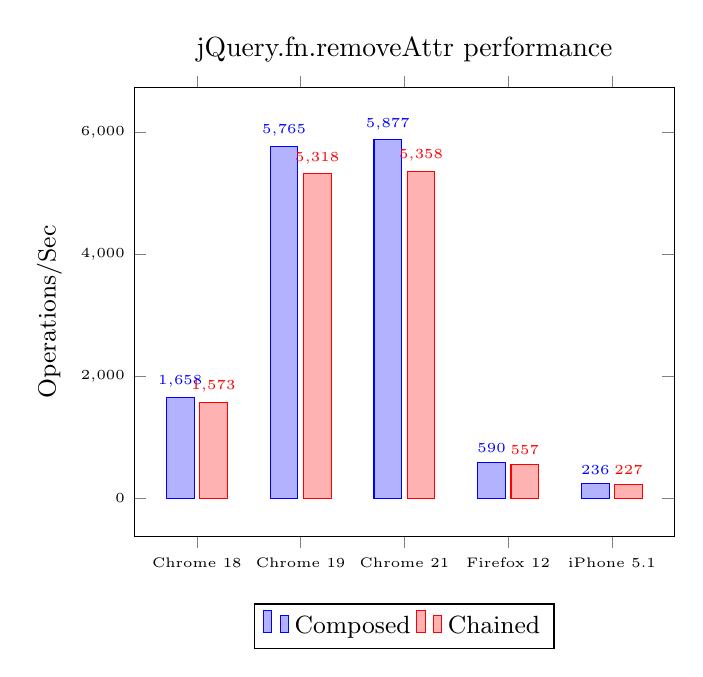
\begin{tikzpicture}
\begin{axis}[
    ybar,
    enlargelimits=0.15,
    ylabel={Operations/Sec},
    symbolic x coords={Chrome 18, Chrome 19, Chrome 21, Firefox 12, iPhone 5.1},
    legend style={
      at={(0.5,-0.15)},
      anchor=north,legend columns=-1
    },
    legend style={font=\small},
    tick label style={font=\tiny},
    label style={font=\small},
    nodes near coords,
    every node near coord/.append style={font=\tiny},
    title=jQuery.fn.removeAttr performance
  ]

\addplot coordinates{
    (Chrome 18, 1658)
    (Chrome 19, 5765)
    (Chrome 21, 5877)
    (Firefox 12, 590)
    (iPhone 5.1, 236)
  };

\addplot coordinates{
    (Chrome 18, 1573)
    (Chrome 19, 5318)
    (Chrome 21, 5358)
    (Firefox 12, 557)
    (iPhone 5.1, 227)
  };

\legend{Composed, Chained}

\end{axis}
\end{tikzpicture}

\section{Relaxing The Functor Definition}

[\textbf{TODO}] Disucss using methods in serial instead of the cmps operation. Discuss the reality of side effects as it relates to preserving identity and composition. Discuss method chains as composition to avoid extra function call overhead which represents the real performance win here.

\section{Haskell's List Functor}

[\textbf{TODO}] Discuss the relationship here with fmap and haskell's list functor. jQuery's objec-set behavior is clearly a list. Cite previous work in that area as an influence.

\section{Guidelines to Facilitate Optimization}

Given that the loop fusion optimization requires the composition of at least two morphisms from \textbf{Html} and that functionality of those morphisms is always provided to the end user as the lifted version that exists in \textbf{Jqry}, we propose the following guidelines.

\begin{enumerate}
  \item \label{item:standard-1} All methods defined on the jQuery object prototype \verb|jQuery.fn| that leverage \verb|jQuery.map| to lift an \textbf{Html} morphism into \textbf{Jqry} must provide the underlying morphism as a property for end users. Since the behavior of a given jQuery method is often too complex for the end user to determine if it meets the criteria for loop fusion, this rightly places the onus on the developers of the jQuery methods to determine and provide the necessary JavaScript function to the end user for optimization in their applications.
  \item \label{item:standard-2} All properties defined for this purpose should exist on the jQuery method itself to avoid confusion among users wishing to optimize their method chains. We propose \verb|composable| as the property name. This guarantees that jQuery methods remain the discreet units of functionality extension that they are today, and the proposed property name is semantically useful.
  \item \label{item:standard-3}Developers should, wherever possible, document and test both the \textbf{Html} morphism and its \textbf{Jqry} incarnation as discrete pieces of functionality to ensure that each \textbf{Html} morphism works independent of its \textbf{Jqry} counterpart. This ensures that the individual properties of both the \textbf{Jqry} and \textbf{Html} morphisms will persist across revisions to both.
\end{enumerate}

To assist jQuery method developers in effecting the above we also propose a small helper function that properly applies \verb|map| to an \textbf{Html} morphism, properly forwards arguments in addition to the initial \textbf{HTMLElement} argument, and sets the \verb|composable| attribute. See Appendix C.

\section{Library Aided Optimization} \label{sec:library-aided-optimization}

The reader will note that the guidelines do not attempt to differentiate the optimizable jQuery methods in any appreciable fashion other than the the possible existence of the \verb|composable| property. This is a deliberate omission in preference to an automatic identification of chains with two or more methods that define the \verb|composable| property. In fact it is possible to automatically fuse the underlying JavaScript functions but this incurs a small additional cognitive overhead and an as yet unresolved performance degradation (See Appendix D).
\\

[\textbf{TODO}] further discuss automatic fusion and possible benefits to end users.

[\textbf{TODO}] explore the reasons for the performance degredation with the automatic approach as it may be relevant to the hand fused approach.
\\

Instead we propose a small library that will log a warning any time two or more methods are invoked in sequence when each provides the \verb|composable| property. Additionally, it will log a warning when two or more of these methods occur in a method chain but are not adjacent. While more detail on one possible implementation is provided in Appendix E, a short explanation here may aid interested parties in creating their own implementation.

Newly instantiated jQuery objects derive the bulk of their functionality from the \verb|jQuery.fn| object defined as their prototype. \verb|jQuery.fn| is also the object onto which new jQuery methods, or \textbf{Jqry} morphisms, are defined. Consequently it's possible to create a proxy object that can be inserted between a jQuery instance and \verb|jQuery.fn| in the prototype chain at runtime to record the sequence of method invocations and report opportunities for optimization.

\begin{figure}[!ht]
\begin{equation} \label{eq:jquery-default}
 jQuery \xrightharpoonup{\ \ f\ \ } jQuery.fn
\end{equation}
\begin{equation} \label{eq:jquery-with-proxy}
 jQuery \xrightharpoonup{\ \ f\ \ } Proxy \xmapsto{\ \ f\ \ } jQuery.fn
\end{equation}
\end{figure}

[\textbf{TODO}] add diagram to illustrate prototype chain alteration
\\

Taking \begin{math}\xrightharpoonup{f}\end{math} to represent the automatic prototype look-up of \begin{math}f\end{math} on the target, and \begin{math}\xmapsto{f}\end{math} to represent a invocation of \begin{math}f\end{math} on the target by the source object we have diagram \ref{eq:jquery-default} as the default jQuery behavior and diagram \ref{eq:jquery-with-proxy} as the desired behavior.

The \begin{math}Proxy\end{math} object must define it's own version of each and every function property of the \begin{math}jQuery.fn\end{math} prototype object. This allows it to count invocations of those functions and for any count greater than one raise a warning. It also allows it to invoke the method of the same name on the \begin{math}jQuery.fn\end{math} when no count is recorded, IE \begin{math}\xmapsto{f}\end{math}. Additionally the size of the jQuery object-set can be taken into account as part of configuration, as small sets of objects won't see the same benefits from composition.

The primary advantage of this approach is that it is entirely unobtrusive and requires nothing more than the inclusion of the library in an HTML document following the inclusion of jQuery itself. In this way it encourages developer adoption through ease of use.

\section{jQuery Project Results}

[\textbf{TODO}] discuss standard with jQuery core team, push for implementation in core. Talk submitted to jQuery Conference in June 2012 with this goal in mind

\section{Client Project Results}

[\textbf{TODO}] discuss implementation with subject application creators using jQuery. Candidates: Originate Labs, The Filament Group, Append To, Bocoup, Adobe

\section{Further Work}

[\textbf{TODO}] discuss further work in applying other category theoretic constructs to the two categories defined here. eg, jQuery is a Monoid, examine cartesian closed categories.

\section{Conclusion}

Here we have clearly defined a common idiom in JavaScript using the jQuery library that can be targeted for performance optimization with a minimum of effort by developers. In addition we have established a small set of guidelines that jQuery extenders and plug-in authors can use to assist the consumers of their software in performing this optimization and provided the framework for an unobtrusive library that can automatically identify areas of potential performance degradation. In future work we hope to pursue the automatic optimization of jQuery method chains using lazy semantics to further reduce developer involvement while continuing to realize the advantages of loop fusion.

\appendix
\section{Appendix A: Each-form}

Another equally popular form of jQuery method construction leverages the jQuery built-in \verb|each| method. Converting the example from Figure \ref{fig:map-form} yields Figure \ref{fig:each-form}. The key difference being the expectation that a side effect will result from the closure that somehow leverages the information of the index and/or the \textbf{HTMLElement}.

\begin{figure}[!ht]
\small
\begin{verbatim}
jQuery.fn.eachForm = function(){
  return this.each(function( index, htmlElement ) {
    // some side effectful computation
  });
};
\end{verbatim}
\nocaptionrule \caption{General each-form}
\label{fig:each-form}
\end{figure}

\section{Appendix B: Composition of Html Morphisms}

Examples of what composition of \textbf{Html} morphisms will look like can server to reassure the reader that it behaves as necessary. In Figure \ref{fig:html-compose} an anchor element has its \verb|foo| and \verb|baz| attributes set by the newly composed \textbf{Html} morphism.

\begin{figure}[!ht]
\small
\begin{verbatim}
function a( elem ){
  elem.setAttribute( "foo", "bar" );
  return elem;
}

function b( elem ){
  elem.setAttribute( "baz", "bak" );
  return elem;
}

var elem = document.getElementById( "example-anchor" );
elem.getAttribute( "foo" ); // undefined
elem.getAttribute( "baz" ); // undefined

elem = compose( a, b )( elem );
elem.getAttribute( "foo" ); // "bar"
elem.getAttribute( "baz" ); // "bak"
\end{verbatim}
\nocaptionrule \caption{Preserving identity and composition}
\label{fig:html-compose}
\end{figure}

\section{Appendix C: Mapable Helper Function}

The \verb|jQuery.mapable| helper described in Figure \ref{fig:mapable} provides a function that can be assigned to a property on the \verb|jQuery.fn| object. It also ``tags'' the function by setting its \verb|composable| attribute to the original \textbf{Html} morphism thereby alerting developers and any libraries wishing to track optimizable \textbf{Jqry} morphisms. Additionally it does the work of forwarding any and all arguments as additional parameters to the \textbf{Html} morphism.

\begin{figure}[!ht]
\small
\begin{verbatim}
jQuery.mapable = function( htmlMorphism ){
  var jqryMorphism = function(){
    var args = arguments;

    jQuery.map(this, function( elem ){
      var newArgs = Array.prototype.slice( args );
      newArgs.unshift(elem);
      htmlMorphism.apply( elem, newArgs );
    });
  };

  jqryMorphism.composable = htmlMorphism;
  return jqryMorphism;
}j
\end{verbatim}
\nocaptionrule \caption{The mapable helper function}
\label{fig:mapable}
\end{figure}

\section{Appendix D}

An initial attempt was made to alter jQuery to support the deferral of method execution until being forced. The idea was to accumulate method calls that defined the \verb|composable| property (\verb|htmlMorphism| in the source) and then do the composition and execution all at once when necessary. While this is possible in JavaScript, the performance overhead of forwarding arguments for method invocations like those in Figure \ref{fig:args-juggle} down to the \textbf{Html} morphism in conjunction with the capability of modern JavaScript virtual machines to compile simple loops to machine code negated any positive effect of limiting the total iterations. You can view the results of a simple performance test at \href{http://jsperf.com/lazy-loop-fusion-vs-traditional-method-chaning/5}{jsperf.com}. You can also view the extension required to effect the lazy optimization at \href{https://github.com/johnbender/jquery-lazy-proxy/blob/79ab61e22547169d6f392512f782df2e29362ebc/lazy.js}{github.com}. Further work and testing is required to completely rule out the possibility of this approach

\begin{figure}[!ht]
\small
\begin{verbatim}
jQuery( "div" ).foo( "bar", "baz" ).force();
\end{verbatim}
\nocaptionrule \caption{Forwarding string arguments}
\label{fig:args-juggle}
\end{figure}

\section{Appendix E}

A basic implementation of the object proxy described in Section \ref{sec:library-aided-optimization} can be found at \href{https://github.com/johnbender/jquery-lazy-proxy/blob/79ab61e22547169d6f392512f782df2e29362ebc/lazy.js}{GitHub} along with a simple counting and logging mechanism for identifying possible optimizations.

\bibliographystyle{abbrvnat}

% The bibliography should be embedded for final submission.

\begin{thebibliography}{}
\softraggedright

\bibitem{bib:usage}
  BuiltWith.com,
  jQuery Usage Statistics,
  \url{http://blog.builtwith.com/2011/10/31/jquery-version-and-usage-report/}
\bibitem{bib:chaining}
  jQuery.com,
  Plugin Authoring,
  Maintaining Chainability,
  \url{http://docs.jquery.com/Plugins/Authoring#Maintaining_Chainability}
\bibitem{bib:category-definition}
  Benjamin C. Pierce,
  \emph{Basic Category Theory for Computer Scientists}.
  MIT Press, Massachusets,
  First Edition,
  1991.
\bibitem{bib:dom}
  www.w3.org,
  Document Object Model (DOM) Level 3 Core Specification,
  \url{http://dev.w3.org/html5/spec/elements.html}
\bibitem{bib:htmlelement}
  W3.org,
  HTMLElement interface specification,
  \url{http://dev.w3.org/html5/spec/elements.html#htmlelement}
\bibitem{bib:all-htmlelements}
  W3.org,
  HTMLElement list,
  \url{http://dev.w3.org/html5/markup/elements.html#html-elements}
\bibitem{bib:deforestation}
  P Wadler,
  \emph{Deforestation: Transforming programs to eliminate trees}.
  Theoretical computer science,
  Elsevier,
  1990.

\end{thebibliography}

\end{document}
